\documentclass[a4paper, 11pt]{article}
\usepackage[italian]{babel}
\usepackage[utf8]{inputenc}
\usepackage{amsmath}
\usepackage{imakeidx}
\usepackage{amsfonts}
\usepackage{amssymb}
\usepackage{float}
\usepackage{graphicx}
\usepackage{caption}
\usepackage[paper=a4paper]{geometry}
\usepackage[shortlabels]{enumitem}
\usepackage{hyperref}
\usepackage{fancyhdr} % <-- aggiunto
\pagestyle{fancy}     % <-- imposto lo stile fancy
\fancyhf{}
\rhead{\includegraphics[width=1cm]{Immagini/Logo_Università_di_Udine.png}} % <-- logo in alto a destra
\hypersetup{
    colorlinks,
    citecolor=black,
    filecolor=black,
    linkcolor=black,
    urlcolor=black
}

% --- INIZIO SOSTITUZIONE MINTED CON LISTINGS ---
\usepackage{listings}
\usepackage{xcolor} % Necessario per definire i colori

\definecolor{codegray}{gray}{0.95}
\definecolor{codegreen}{rgb}{0.0, 0.5, 0.0} % Per i commenti
\definecolor{codered}{rgb}{0.9, 0.0, 0.0}   % Per le stringhe
\definecolor{codeblue}{rgb}{0.0, 0.0, 0.9}   % Per le parole chiave

\lstdefinestyle{mycodestyle}{
    backgroundcolor=\color{codegray}, % Colore di sfondo
    basicstyle=\small\ttfamily,       % Stile del testo del codice (dimensione piccola, font a spaziatura fissa)
    breaklines=true,                  % Permette al codice di andare a capo
    frame=single,                     % Aggiunge un bordo singolo
    framesep=5pt,                     % Spazio tra il bordo e il codice
    framerule=0.5pt,                  % Spessore del bordo
    rulecolor=\color{orange!70},     % Colore del bordo (arancione come nel tuo esempio)
    numbers=left,                     % Numerazione delle righe a sinistra
    numberstyle=\tiny\color{gray},    % Stile dei numeri di riga
    stepnumber=1,                     % Incremento dei numeri di riga
    numbersep=8pt,                    % Spazio tra numeri e codice
    showspaces=false,                 % Non mostrare spazi come simboli
    showtabs=false,                   % Non mostrare tab come simboli
    showstringspaces=false,           % Non mostrare spazi nelle stringhe
    commentstyle=\color{codegreen}\textit, % Stile per i commenti (verde, corsivo)
    keywordstyle=\color{codeblue}\bfseries, % Stile per le parole chiave (blu, grassetto)
    stringstyle=\color{codered},      % Stile per le stringhe (rosso)
    % Se vuoi un titolo/didascalia per il blocco di codice, potresti usare captionpos, ad esempio:
    % captionpos=b, % didascalia sotto
    % caption={Descrizione del codice},
}
% --- FINE SOSTITUZIONE MINTED CON LISTINGS ---


\renewcommand{\contentsname}{Indice}
\title{Laboratorio di Algoritmi e Strutture Dati\\A.A. 2024/25}
\author{Andrea Gioia - 169484@spes.uniud.it\\Luca Gamberini - 168712@spes.uniud.it}

\begin{document}

\maketitle
\tableofcontents
\newpage
\section{Introduzione}
Il progetto include le misurazioni e la conseguente graficazione di 4 algoritmi di ordinamento:
\begin{itemize}
    \item QuickSort
    \item QuickSort 3 Way
    \item CountingSort
\end{itemize}
\subsection{Specifiche tecniche}
Le specifiche tecniche delle misurazioni sono state:
\begin{itemize}
    \item Array generato con valori decimali \textbf{casuali}
    \item La lunghezza dell'array è compresa tra 100 e 100 mila valori
    \item Il valore di ciascun elemento dell'array varia casualmente tra 10 e un milione
\end{itemize}
Gli algoritmi sono stati implementati in linguaggio Python, mentre le misurazioni dei tempi sono state prese tramite la funzione \href{https://docs.python.org/3/library/time.html#time.perf_counter}{\textit{\texttt{perf\char`_counter}}} della libreria \textit{time}

\section{Algoritmi}
Gli algoritmi di ordinamento presi in esame presentano caratteristiche differenti e risultano più o meno efficienti in base alle carattestiche dell'array di elementi da ordinare.

\subsection{QuickSort}
Algoritmo di ordinamento ricorsivo del tipo divide-et-impera, quindi basato sulla suddivisione in n sottoproblemi, risolti ricorsivamente, fino al raggiungimento del caso base.\\
Non presenta la necessità di utilizzo di strutture dati aggiuntive, di conseguenza lo scambio di elementi avviene in-place.\\\\
Le complessità asintotiche temporali di QuickSort sono:
\begin{itemize}
    \item Caso ottimo: $\Omega(n\log_2n)$
    \item Caso medio: $\Theta(n\log_2n)$
    \item Caso pessimo: $\mathcal{O}(n^2)$
\end{itemize}

\subsubsection{Codice}
\begin{lstlisting}[style=mycodestyle, language=Python]
def QuickSort( A, p, q ):
    if( p < q ):
        r = Partition( A, p, q)
        QuickSort( A, p, r-1 )
        QuickSort( A, r+1, q )
    return A

def Partition(A, p, q):
    x = A[q]
    i = p - 1
    for j in range(p, q):
        if A[j] <= x:   # (corretto A[j], non A[q])
            i += 1
            Scambia(A, i, j)
    Scambia(A, i + 1, q)    # posiziona il pivot al centro
    return i + 1

def Scambia(A, i, j):
    temp = A[i]
    A[i] = A[j]
    A[j] = temp
\end{lstlisting}
---Commento del codice---

\subsection{QuickSort3Way}
Versione modificata rispetto al QuickSort classico.\\
Prevede la suddivisione in 3 parti dell'array di elementi, sulla base di una variabile \textit{pivot}.\\
Gli scambi vengono fatti sulla base di un confronto tra elemento dell'array e la variabile pivot ($>$, $<$, $=$). Le chiamate ricorsive vengono effettuate su porzioni con elementi $<$ pivot e $>$ pivot.\\
A differenza del QuickSort classico, QuickSort3Way presenta notevole efficienza con array con molti elementi duplicati.\\\\
Le complessità asintotiche temporali di QuickSort3Way sono:
\begin{itemize}
    \item Caso ottimo: $\Omega(n\log n)$
    \item Caso medio: $\Theta(n\log n)$
    \item Caso pessimo: $\mathcal{O}(n^2)$
\end{itemize}

\subsubsection{Codice}
\begin{lstlisting}[style=mycodestyle, language=Python]
    def QuickSort3Way(arr, l, r):
    if l >= r:
        return

    lt = l
    i = l
    gt = r
    pivot = arr[l]

    while i <= gt:
        if arr[i] < pivot:
            arr[lt], arr[i] = arr[i], arr[lt]
            lt += 1
            i += 1
        elif arr[i] > pivot:
            arr[i], arr[gt] = arr[gt], arr[i]
            gt -= 1
        else:
            i += 1

    QuickSort3Way (arr, l, lt - 1)
    QuickSort3Way (arr, gt + 1, r)

    return lt, gt
\end{lstlisting}

\subsection{CountingSort}
CountingSort è un algoritmo di ordinamento non in-place, in quanto si avvale di un array aggiuntivo che conta il numero di occorrenze di ciascun elemento.\\\\
Le complessità asintotiche temporali di CountingSort sono:
\begin{itemize}
    \item Caso ottimo: $\Omega(n + k)$
    \item Caso medio: $\Theta(n + k)$
    \item Caso pessimo: $\mathcal{O}(n + k)$
\end{itemize}

\subsubsection{Codice}
\begin{lstlisting}[style=mycodestyle, language=Python]
    def countingSort(arr):
    max = arr[0]
    min = arr[0]

    for i in range(1, len(arr)):
        if arr[i] > max:
            max = arr[i]
        elif arr[i] < min:
            min = arr[i]

    C = [0] * (max - min + 1)
    for i in range(len(arr)):
        C[arr[i] - min] += 1

    k = 0
    for i in range(len(C)):
        while C[i] > 0:
            arr[k] = i + min
            k += 1
            C[i] -= 1
\end{lstlisting}

\subsection{RadixSort}
RadixSort è un algoritmo di ordinamento basato sull'ordinamento cifra per cifra, partendo da quella meno significativa. Risulta particolarmente efficiente in presenta di molti numero con la stessa quantità di cifre.\\\\
Le complessità asintotiche temporali di RadixSort sono:
\begin{itemize}
    \item Caso ottimo: $\Omega(n\cdot d)$
    \item Caso medio: $\Theta(n\cdot d)$
    \item Caso pessimo: $\mathcal{O}(n\cdot d)$
\end{itemize}

\begin{lstlisting}[style=mycodestyle, language=Python]
def RadixSort(arr):
    radix_array = [[], [], [], [], [], [], [], [], [], []]  # array delle cifre
    max_val = max(arr)  # assegno il valore massimo dell'array
    exp = 1 

    while (max_val // exp) > 0:
        while len(arr) > 0:
            val = arr.pop()
            radix_index = (val // exp) % 10
            radix_array[radix_index].append(val)

        for bucket in radix_array:
            while len(bucket) > 0:
                val = bucket.pop()
                arr.append(val)

        exp *= 10
\end{lstlisting}

\section{Misurazioni}

\begin{table} [H]
    \centering
    \begin{tabular}{|c|c|}
        \hline
        QuickSort \\ [0.1 cm]
        \hline
    \end{tabular}
\end{table}

\begin{figure} [H]
    \centering
    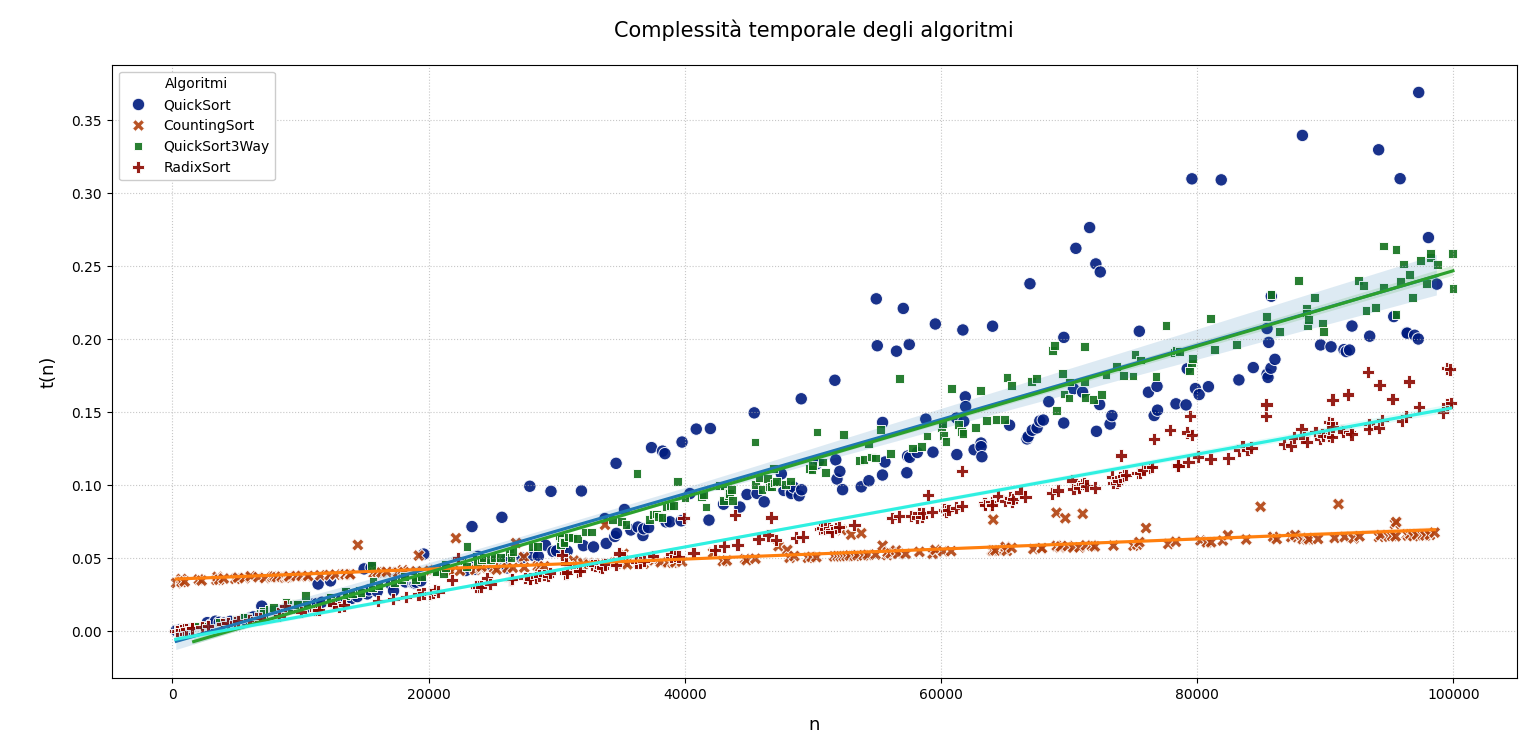
\includegraphics[scale=0.5]{Immagini/Grafico.png}
    \caption*{Parte reale sulle x, parte immaginaria sulle y}
\end{figure}

\section{Conclusione}
Conclusione della relazione.

\end{document}